Die Ortsänderung in einem Zeitabschnitt ist die Fläche zwischen dem $v(t)$-Graphen und der $t$-Achse, über der Achse positiv, unter der Achse negativ.
\begin{center}
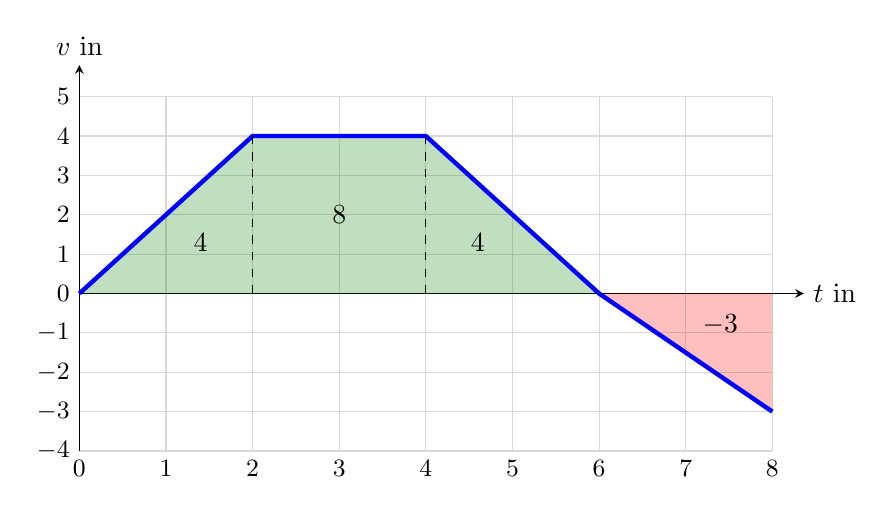
\begin{tikzpicture}[>=stealth, x=1.1cm, y=0.5cm]
 \draw[gray!30] (0,-4) grid[xstep=1, ystep=1] (8,5);
 \draw[->] (0,0) -- (8.364,0) node[right] {$t$ in \si{\second}};
 \draw[->] (0,-4) -- (0,5.8) node[above] {$v$ in \si{\meter\per\second}};
 \foreach \tk in {0,1,2,3,4,5,6,7,8} \node[below] at (\tk,-4) {\small $\tk$};
 \foreach \yk in {-4,-3,-2,-1,0,1,2,3,4,5} \node[left] at (0,\yk) {\small $\yk$};

 \fill[green!50!black, opacity=0.25] (0,0) -- (2,4) -- (4,4) -- (6,0) -- cycle;
 \fill[red, opacity=0.25] (6,0) -- (8,-3) -- (8,0) -- cycle;
 \draw[ultra thick, blue] (0,0) -- (2,4) -- (4,4) -- (6,0) -- (8,-3);
 \draw[dashed] (2,0) -- (2,4) (4,0) -- (4,4);
 \node at (1.4,1.3) {$4$};
 \node at (3,2) {$8$};
 \node at (4.6,1.3) {$4$};
 \node at (7.4,-0.8) {$-3$};
\end{tikzpicture}
\end{center}
\begin{align}
 \Delta s_1 &= \dOneF = \dOne \\
 \Delta s_2 &= \dTwoF = \dTwo \\
 \Delta s_3 &= \dThreeF = \dThree \\
 \Delta s_4 &= \dFourF = \dFour
\end{align}
\begin{abcliste}
\abc Bis \tThreeO\ ist $v>0$, der Körper entfernt sich vom Start; danach ist $v<0$, er fährt zurück. Am weitesten entfernt ist er also bei $\result{t = \tThreeO}$:
\begin{align}
 s_\mathrm{max} &= \sMaxF = \sMax \approx \result{\sMaxP{0}{2}}
\end{align}
\abc Die Ortsänderung ist die Summe der Flächen mit Vorzeichen:
\begin{align}
 \Delta s &= \displF = \displ \approx \result{\displP{0}{2}}
\end{align}
\abc Für die zurückgelegte Strecke zählt auch der Rückweg positiv:
\begin{align}
 d &= \distF = \dist \approx \result{\distP{0}{2}}
\end{align}
Der Körper fährt \sMaxP{0}{2} vorwärts und \SI{3}{\meter} zurück: Er legt \distP{0}{2} zurück, ist am Ende aber nur \displP{0}{2} vom Start entfernt.
\end{abcliste}
